\begin{frame}
	\frametitle{Projektverlauf\hfill{}\footnotesize \group}
	\framesubtitle{Visualisierung mit gource}
	\begin{columns}
		\begin{column}{0.5\textwidth}
			\begin{block}{Gerenderte Animation von github.com/accefa/doku}
				\movie[width=4cm,height=4cm, externalviewer]{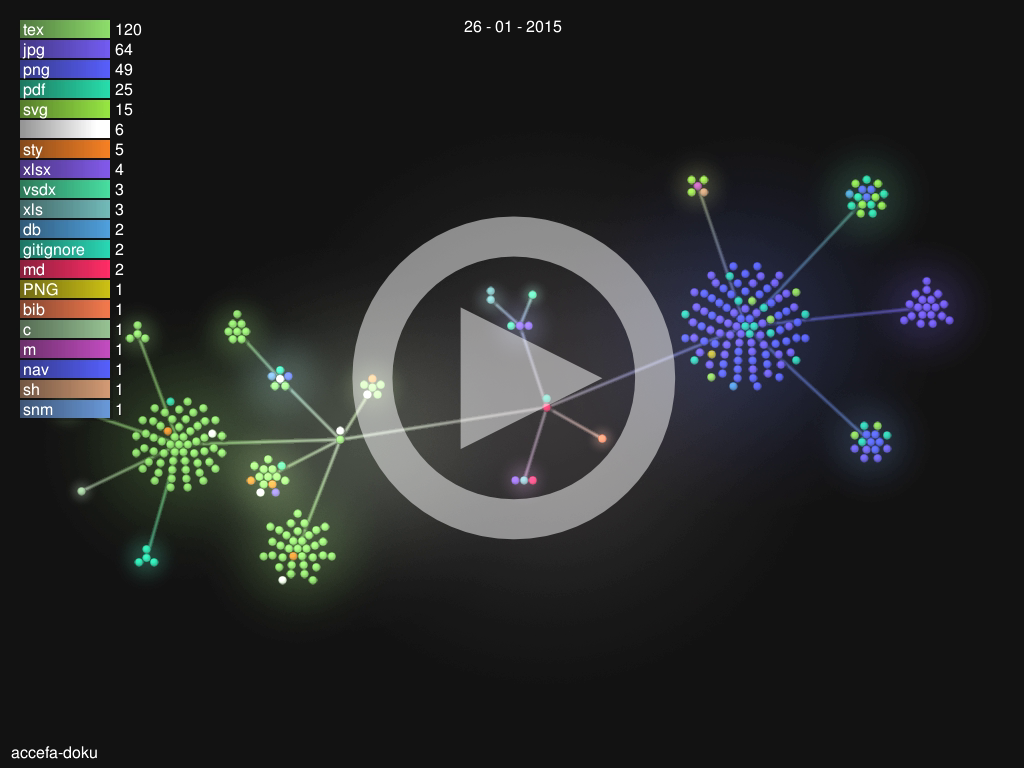
\includegraphics[width=1\textwidth]{../../fig/gource_play.png}}{gource-dark.mp4}
				\\ gource-dark.mp4 \hfill{} 1:24 min
			\end{block}
		\end{column}
		\begin{column}{0.5\textwidth}
			\begin{exampleblock}{gource Parameter}
				\lstinputlisting{gource-commands.txt}
			\end{exampleblock}
		\end{column}
	\end{columns}
\end{frame}

\begin{frame}
	\frametitle{Projektmanagement \hfill{} \footnotesize \group}
	\framesubtitle{Regelkreis für Arbeitspakete}
	\begin{figure}
		\begin{tikzpicture}[node distance=2.85cm, scale=0.75, transform shape]
			\footnotesize
			\node (m) [flowchart-block] {define Milestone};
			\node (i) [flowchart-block, right of=m] {define Issue};
			\node (a) [flowchart-block, right of=i] {(re)assign Member};
			\node (ov) [flowchart-decision, below right of=a] {Assignee overload?};
			\node (si) [flowchart-block, right of=ov] {solve Issue};
			\node (is) [flowchart-decision, below of=si] {Issue solved?};
			\node (ci) [flowchart-block, right of=is] {close Issue};
			\node (np) [flowchart-decision, below of=i] {new problem?};
			\draw[blue, thick, ->] (m) -- (i);
			\draw[blue, thick, ->] (i) -- (a);
			\draw[blue, thick, ->] (a) -| (ov);
			\draw[blue, thick, ->] (ov) -| node[anchor=south, near start] {yes} (a);
			\draw[blue, thick, ->] (ov) -- node[anchor=south, near start] {no} (si);
			\draw[blue, thick, ->] (si) -- (is);
			\draw[blue, thick, ->] (is) -- node[anchor=south, near start] {yes} (ci);
			\draw[blue, thick, ->] (is) -| node[anchor=south, near start] {no} (np);
			\draw[blue, thick, ->] (np) -| node[anchor=south, near start] {no} (a);
			\draw[blue, thick, ->] (np) -- node[anchor=west, near start] {yes} (i);
		\end{tikzpicture}
	\end{figure}
\end{frame}

\subsubsection{Fachgruppe ET}
\begin{frame}
	\frametitle{Fachgruppe Elektrotechnik\hfill{}\footnotesize \group}
	\framesubtitle{Motivation \& Ziele}
	\begin{columns}
		\begin{column}{0.5\textwidth}
				\textit{``Denn es ist eines ausgezeichneten
					Mannes nicht würdig, wertvolle Stunden
					wie ein Sklave im Keller der einfachen
					Berechnungen zu verbringen''}
				~ \\ ~ \\
				\hfill{} -- Gottfried Wilhelm Leibniz \\
		\end{column}
		\pause
		\begin{column}{0.5\textwidth}
			\begin{block}{Ziele}
				\begin{itemize}
					\item Synergien nutzen
					\item Fachlicher Austausch
					\item Eigenentwicklungen
					\item OpenHardware
				\end{itemize}
			\end{block}
		\end{column}
	\end{columns}
\end{frame}

\begin{frame}
	\frametitle{Fachgruppe Elektrotechnik \hfill{} \footnotesize \group}
	\framesubtitle{Organisation \& Projekte}
	\begin{columns}
		\begin{column}{0.5\textwidth}
			\begin{block}{github.com/pren-et}
				\begin{itemize}
					\item 7 Contributors
					\item 6 PREN-Teams
					\item 7 Repositories
					\item 3 HW-Projekte
				\end{itemize}
			\end{block}
			\begin{block}{Projekte}
				\begin{itemize}
					\item Motorentreiber für
						\begin{itemize}
							\item Gleichstrommotor (DC)
							\item Brushlessmotor (BLDC)
							\item Schrittmotor (Stepper)
						\end{itemize}
					\item Dokumentationen
				\end{itemize}
			\end{block}
		\end{column}
		\begin{column}{0.5\textwidth}
			\begin{exampleblock}{Teams}
				\begin{tabular}{l l r}
					DC
						& B. v. Büren 	& 19 \\
						& J. Buchli 	& 19 \\
						& F. Kreiliger	& 33 \\
						& E. Mazlagi\'c	& 39 \\
					& & \\
					BLDC
						& D. Winz	& 27 \\
						& Y. Studer	& 32 \\
					& & \\
					Stepper
						& D. Winz	& 27 \\
						& F. Kreiliger	& 33 \\
						& B. Wyss	& 38 \\
				\end{tabular}
			\end{exampleblock}
		\end{column}
	\end{columns}
\end{frame}
